\documentclass[12pt,a4paper]{article}

% ─── Page Layout ───────────────────────────────────────────────────────────────
\usepackage[a4paper, margin=0.8in, headheight=14pt]{geometry}

% ─── Fonts (XeLaTeX) ───────────────────────────────────────────────────────────
\usepackage{fontspec}
\usepackage{unicode-math}
\setmainfont{TeX Gyre Pagella}
\setmonofont[Scale=0.88]{TeX Gyre Cursor}
\setmathfont{Latin Modern Math}

% ─── Packages ──────────────────────────────────────────────────────────────────
\usepackage{xcolor}
\usepackage{colortbl}
\usepackage{titlesec}
\usepackage{enumitem}
\usepackage{tabularx}
\usepackage{booktabs}
\usepackage{array}
\usepackage{amsmath}
\usepackage{tikz}
\usetikzlibrary{shapes.geometric, arrows.meta, positioning, calc, fit, decorations.pathreplacing, decorations.pathmorphing}
\usepackage{tcolorbox}
\tcbuselibrary{skins, breakable}
\usepackage{hyperref}
\usepackage{fancyhdr}
\usepackage{graphicx}
\usepackage{microtype}
\hyphenpenalty=10000
\exhyphenpenalty=10000
\sloppy
\usepackage{caption}
\usepackage{setspace}
\usepackage{multirow}
\usepackage{tocloft}

% ─── Q&A helper ────────────────────────────────────────────────────────────────
\newcommand{\Q}[1]{\textbf{#1}\par\noindent\ignorespaces}

% ─── Colour Palette ────────────────────────────────────────────────────────────
\definecolor{myred}{RGB}{196,30,58}
\definecolor{mydark}{RGB}{30,30,50}
\definecolor{mygreen}{RGB}{14,120,80}
\definecolor{myteal}{RGB}{0,130,140}
\definecolor{myamber}{RGB}{180,100,0}
\definecolor{mypurple}{RGB}{100,30,160}
\definecolor{mygray}{RGB}{246,247,249}
\definecolor{mgframe}{RGB}{180,185,200}
\definecolor{watermark}{RGB}{145,150,170}
\definecolor{hdrred}{RGB}{250,232,235}
\definecolor{hdrgreen}{RGB}{220,244,233}
\definecolor{hdrteal}{RGB}{220,242,244}
\definecolor{hdramber}{RGB}{253,242,215}
\definecolor{hdrpurple}{RGB}{238,228,255}
\definecolor{hdrgray}{RGB}{238,240,245}
\definecolor{rowalt}{RGB}{250,251,253}

% ─── Section Formatting ────────────────────────────────────────────────────────
\titleformat{\section}
  {\large\bfseries\color{myred}}{\thesection.}{0.5em}{}
  [\vspace{1pt}{\color{myred}\rule{\linewidth}{0.8pt}}]
\titleformat{\subsection}
  {\normalsize\bfseries\color{myteal}}{\thesubsection}{0.5em}{}
\titlespacing*{\section}{0pt}{18pt}{7pt}
\titlespacing*{\subsection}{0pt}{11pt}{4pt}

% ─── Paragraph ─────────────────────────────────────────────────────────────────
\setlength{\parindent}{0pt}
\setlength{\parskip}{4pt}

% ─── TOC Styling ───────────────────────────────────────────────────────────────
\renewcommand{\cfttoctitlefont}{\large\bfseries\color{myred}}
\renewcommand{\cftaftertoctitle}{\par\noindent{\color{myred}\rule{\linewidth}{0.8pt}}}
\setlength{\cftbeforetoctitleskip}{0pt}
\setlength{\cftaftertoctitleskip}{6pt}
\renewcommand{\cftsecfont}{\normalsize\bfseries\color{mydark}}
\renewcommand{\cftsecpagefont}{\normalsize\bfseries\color{mydark}}
\renewcommand{\cftsecleader}{\cftdotfill{\cftdotsep}}
\setlength{\cftbeforesecskip}{7pt}
\renewcommand{\cftsubsecfont}{\small\color{mydark}}
\renewcommand{\cftsubsecpagefont}{\small\color{mydark}}
\setlength{\cftbeforesubsecskip}{3pt}
\setlength{\cftsubsecindent}{1.4em}

% ─── Table helpers ─────────────────────────────────────────────────────────────
\renewcommand{\arraystretch}{1.45}
\setlength{\tabcolsep}{6pt}
\arrayrulecolor{mydark}
\newcolumntype{B}[1]{>{\small\bfseries\raggedright\arraybackslash}m{#1}}
\newcolumntype{C}[1]{>{\centering\arraybackslash}m{#1}}
\newcolumntype{Y}{>{\small\raggedright\arraybackslash}X}
\renewcommand{\tabularxcolumn}[1]{m{#1}}

% ─── Header / Footer ───────────────────────────────────────────────────────────
\pagestyle{fancy}
\fancyhf{}
\fancyhead[L]{\small\color{myred}\textbf{OE-EC704A}\;\color{mydark}--- Web Technology}
\fancyhead[R]{\small\color{myteal}\textbf{Module 4 Notes}}
\fancyfoot[C]{\small\color{mydark}\thepage}
\fancyfoot[R]{\small\color{watermark}\textit{\copyright\ Biraj}}
\renewcommand{\headrulewidth}{0.5pt}
\renewcommand{\footrulewidth}{0.3pt}

% ─── Hyperref ──────────────────────────────────────────────────────────────────
\hypersetup{
  colorlinks=true, linkcolor=myteal, urlcolor=myteal,
  pdfauthor={Biraj Sarkar},
  pdftitle={OE-EC704A --- Module 4 Notes}
}

% ─── tcolorbox styles ──────────────────────────────────────────────────────────
\tcbset{
  tikzbox/.style={
    colback=mygray, colframe=mgframe, boxrule=0.6pt, arc=4pt,
    left=8pt, right=8pt, top=6pt, bottom=6pt,
    colbacktitle=mgframe, coltitle=mydark,
    fonttitle=\small\bfseries
  },
  defbox/.style={
    colback=hdrgreen, colframe=mygreen, boxrule=0.8pt, arc=4pt,
    left=9pt, right=9pt, top=6pt, bottom=6pt,
    colbacktitle=mygreen, coltitle=white,
    fonttitle=\small\bfseries
  },
  formulabox/.style={
    colback=hdrteal, colframe=myteal, boxrule=0.8pt, arc=4pt,
    left=9pt, right=9pt, top=7pt, bottom=7pt,
    colbacktitle=myteal, coltitle=white,
    fonttitle=\small\bfseries
  },
  examplebox/.style={
    colback=hdramber, colframe=myamber, boxrule=0.8pt, arc=4pt,
    left=9pt, right=9pt, top=6pt, bottom=6pt,
    colbacktitle=myamber, coltitle=white,
    fonttitle=\small\bfseries
  },
  masonbox/.style={
    colback=hdrpurple, colframe=mypurple, boxrule=0.8pt, arc=4pt,
    left=9pt, right=9pt, top=6pt, bottom=6pt,
    colbacktitle=mypurple, coltitle=white,
    fonttitle=\small\bfseries
  },
  exambox/.style={
    colback=hdrpurple, colframe=mypurple, boxrule=1pt, arc=5pt,
    left=10pt, right=10pt, top=8pt, bottom=8pt,
    colbacktitle=mypurple, coltitle=white,
    fonttitle=\bfseries,
    breakable, title after break={\textbf{Frequently Asked / Viva Questions (contd.)}}}
}
\tcbset{breakable}

% ─── TikZ styles ───────────────────────────────────────────────────────────────
\tikzset{
  block/.style={rectangle, draw=myteal, fill=hdrteal,
    text width=2.5cm, align=center, minimum height=1.0cm,
    font=\small, rounded corners=3pt, line width=0.7pt},
  redblock/.style={rectangle, draw=myred, fill=hdrred,
    text width=2.5cm, align=center, minimum height=1.0cm,
    font=\small, rounded corners=3pt, line width=0.7pt},
  netnode/.style={rectangle, draw=myteal, fill=hdrteal,
    text width=1.8cm, align=center, minimum height=0.8cm,
    font=\small, rounded corners=3pt, line width=0.7pt},
  sumjunc/.style={circle, draw=myamber, fill=hdramber,
    minimum size=0.6cm, font=\small, line width=0.8pt},
  snode/.style={circle, draw=mypurple, fill=hdrpurple,
    minimum size=0.55cm, font=\footnotesize, line width=0.7pt},
  arrow/.style={-Stealth, thick, color=mydark},
  redarrow/.style={-Stealth, thick, color=myred},
  line/.style={thick, color=mydark}
}

% ═══════════════════════════════════════════════════════════════════════════════
\begin{document}
% ═══════════════════════════════════════════════════════════════════════════════

\begin{center}
  {\LARGE\bfseries\color{myred} OE-EC704A --- Web Technology}\\[5pt]
  {\normalsize\color{mydark} Semester VII \quad$\bullet$\quad 3L:0T:0P \quad$\bullet$\quad 3 Credits}\\[3pt]
  {\normalsize\color{myteal}\textbf{Module 4 Exam Notes: Exception Handling, Strings, I/O Streams \& Collections}}\\[3pt]
  {\small\color{mydark} CGEC \;$|$\; B.Tech ECE (2023--27) \;$|$\; \textit{Biraj Sarkar}}
\end{center}
\vspace{2pt}
\noindent{\color{myred}\rule{\linewidth}{1.5pt}}
\vspace{2pt}

\hypersetup{linkcolor=mydark}
\tableofcontents
\hypersetup{linkcolor=myteal}
\newpage

% ===============================================================================
\section{Java Exception Handling Mechanism}
% ===============================================================================

An exception is an event that disrupts the normal flow of instruction execution. Java uses a structured exception handling system based on five keywords: \texttt{try}, \texttt{catch}, \texttt{throw}, \texttt{throws}, and \texttt{finally}.

\begin{tcolorbox}[defbox, title={\textbf{Exception Types}}]
\begin{itemize}[leftmargin=*, itemsep=3pt]
  \item \textbf{Checked Exceptions (Compile-time):} Exceptions that must be declared in the method signature or handled in a try-catch block. Verified by the compiler (e.g., \texttt{IOException}, \texttt{SQLException}).
  \item \textbf{Unchecked Exceptions (Runtime):} Exceptions that extend \texttt{RuntimeException}. Not verified by the compiler (e.g., \texttt{NullPointerException}, \texttt{ArithmeticException}).
  \item \textbf{Errors:} Serious conditions that applications should not try to catch. They represent system failures (e.g., \texttt{OutOfMemoryError}, \texttt{StackOverflowError}).
\end{itemize}
\end{tcolorbox}

\begin{tcolorbox}[tikzbox, title={Java Exception Class Hierarchy}]
\centering
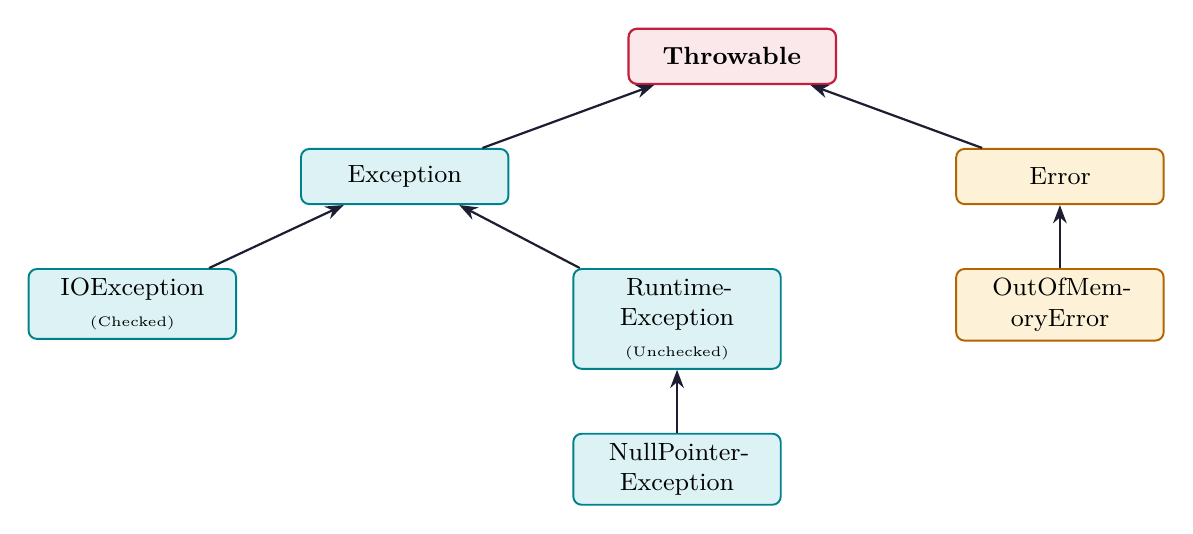
\begin{tikzpicture}[node distance=1.2cm and 1.5cm,
  root/.style={rectangle, draw=myred, fill=hdrred, text width=2.4cm,
    align=center, minimum height=0.7cm, font=\small\bfseries, rounded corners=3pt, line width=0.8pt},
  node/.style={rectangle, draw=myteal, fill=hdrteal, text width=2.4cm,
    align=center, minimum height=0.7cm, font=\small, rounded corners=3pt, line width=0.7pt},
  error/.style={rectangle, draw=myamber, fill=hdramber, text width=2.4cm,
    align=center, minimum height=0.7cm, font=\small, rounded corners=3pt, line width=0.7pt}]

  % Hierarchy Nodes
  \node[root] (throw) {Throwable};
  \node[node, below left=0.8cm and 1.5cm of throw] (ex) {Exception};
  \node[error, below right=0.8cm and 1.5cm of throw] (err) {Error};
  
  \node[node, below left=0.8cm and 0.8cm of ex] (chk) {IOException\\{\tiny (Checked)}};
  \node[node, below right=0.8cm and 0.8cm of ex] (rt) {RuntimeException\\{\tiny (Unchecked)}};
  
  \node[error, below=0.8cm of err] (oome) {OutOfMemoryError};
  \node[node, below=0.8cm of rt] (npe) {NullPointer-\\Exception};

  % Paths
  \draw[arrow] (ex) -- (throw);
  \draw[arrow] (err) -- (throw);
  \draw[arrow] (chk) -- (ex);
  \draw[arrow] (rt) -- (ex);
  \draw[arrow] (npe) -- (rt);
  \draw[arrow] (oome) -- (err);
\end{tikzpicture}
\end{tcolorbox}

\subsection{Checked vs. Unchecked Exceptions}

\par\noindent
{\renewcommand{\arraystretch}{1.5}%
\begin{tabularx}{\linewidth}{|B{3.2cm}|Y|Y|}
\hline
\textbf{Feature} & \textbf{Checked Exceptions} & \textbf{Unchecked Exceptions} \\
\hline
\textbf{Compiler Checks} & Enforced at compilation. & Not verified by the compiler. \\
\hline
\textbf{Base Superclass} & Inherits from \texttt{java.lang.Exception}. & Inherits from \texttt{java.lang.RuntimeException}. \\
\hline
\textbf{Resolution Rule} & Must use \texttt{try-catch} or declare \texttt{throws}. & Recommended to write defensive checks. \\
\hline
\textbf{Examples} & \texttt{FileNotFoundException, IOException} & \texttt{ArithmeticException, NullPointerException} \\
\hline
\end{tabularx}}

% ===============================================================================
\section{Java String Handling}
% ===============================================================================

Java represents sequences of characters using the \texttt{String} class.

\begin{tcolorbox}[defbox, title={\textbf{String Immutability}}]
Java String objects are \textbf{immutable}, meaning their state cannot be modified after creation. 
\begin{itemize}[leftmargin=*, itemsep=3pt]
  \item \textbf{String Pool:} When a string literal is declared, the JVM checks if it exists in the String Constant Pool (SCP) on the heap. If present, it reuses the reference, saving heap memory.
  \item \textbf{Why Immutable?} Ensures thread safety, security (parameters like DB connection URLs cannot be altered), and enables string pool caching.
\end{itemize}
\end{tcolorbox}

\subsection{String vs. StringBuffer}

\par\noindent
{\renewcommand{\arraystretch}{1.5}%
\begin{tabularx}{\linewidth}{|B{3.2cm}|Y|Y|}
\hline
\textbf{Metric} & \textbf{String Class} & \textbf{StringBuffer Class} \\
\hline
\textbf{Mutability} & Immutable (read-only once created). & Mutable (can append or modify content). \\
\hline
\textbf{Performance} & Slower for frequent concatenations (creates new objects). & Fast and memory efficient (modifies local buffer). \\
\hline
\textbf{Thread Safety} & Naturally thread-safe due to immutability. & Thread-safe; methods are synchronized. \\
\hline
\textbf{Heap Allocation} & SCP or standard heap space. & Standard heap space only. \\
\hline
\end{tabularx}}

\subsection{String and StringBuffer Constructors}
Both classes provide multiple constructors to instantiate character sequences:

\par\noindent
{\renewcommand{\arraystretch}{1.45}%
\begin{tabularx}{\linewidth}{|B{3.5cm}|B{3.8cm}|Y|}
\hline
\textbf{Constructor} & \textbf{Signature} & \textbf{Description} \\
\hline
Default String & \texttt{String()} & Initializes a newly created, empty String object. \\
\hline
Char Array String & \texttt{String(char[] value)} & Allocates a new String representing the char array's contents. \\
\hline
String Copier & \texttt{String(String original)} & Initializes a copy of the argument string. \\
\hline
Buffer Converter & \texttt{String(StringBuffer sb)} & Converts a mutable StringBuffer into an immutable String. \\
\hline
Default Buffer & \texttt{StringBuffer()} & Creates an empty buffer with an initial capacity of 16 characters. \\
\hline
Capacity Buffer & \texttt{StringBuffer(int cap)} & Creates an empty buffer with the specified initial capacity. \\
\hline
String Buffer & \texttt{StringBuffer(String str)} & Creates a buffer initialized with the specified string content. \\
\hline
\end{tabularx}}

\subsection{Core String Operations}
The String class provides a rich set of methods for manipulating character sequences. Because String is immutable, all modifying methods return a \textbf{new} String instance representing the result.

\par\noindent
{\renewcommand{\arraystretch}{1.4}%
\begin{tabularx}{\linewidth}{|B{3.0cm}|B{4.5cm}|Y|}
\hline
\textbf{Operation} & \textbf{Key Method Signature} & \textbf{Functional Description} \\
\hline
\textbf{Extraction} & \texttt{char charAt(int index)} & Returns the char value at the specified index ($0$ to $\text{length}-1$). \\
                    & \texttt{int length()} & Returns the number of characters in the string. \\
\hline
\textbf{Comparison} & \texttt{boolean equals(Object obj)} & Compares string values for character-by-character equality. \\
                    & \texttt{boolean equalsIgnoreCase(String s)} & Value comparison ignoring case differences. \\
                    & \texttt{int compareTo(String anotherString)} & Lexicographically compares two strings (returns $0$ if equal, negative if less, positive if greater). \\
\hline
\textbf{Searching}  & \texttt{int indexOf(String str)} & Returns the index of the first occurrence of the substring (or $-1$). \\
                    & \texttt{int lastIndexOf(String str)} & Returns the index of the last occurrence of the substring. \\
                    & \texttt{boolean contains(CharSequence s)} & Returns true if the string contains the specified sequence. \\
\hline
\textbf{Modifying}  & \texttt{String substring(int begin, int end)} & Extracts a new substring from \texttt{begin} (inclusive) to \texttt{end} (exclusive). \\
                    & \texttt{String concat(String str)} & Appends the specified string to the end (equivalent to the \texttt{+} operator). \\
                    & \texttt{String replace(char old, char new)} & Returns a new string with all occurrences of \texttt{old} replaced by \texttt{new}. \\
                    & \texttt{String trim()} & Returns a copy with leading and trailing whitespaces omitted. \\
\hline
\end{tabularx}}

\subsection{Utility Conversions: \texttt{toString()} and \texttt{valueOf()}}
Java provides built-in mechanisms to convert objects and primitive values into string representations:

\begin{itemize}[leftmargin=*, itemsep=3pt]
  \item \textbf{The \texttt{toString()} Method:} Defined in the root \texttt{Object} class. Every class inherits it, and standard library classes (like \texttt{String}, \texttt{StringBuffer}, \texttt{ArrayList}) override it to return a readable value representation. 
  \begin{itemize}[label=\(\circ\), leftmargin=1.5em]
    \item When an object reference is printed via \texttt{System.out.println(obj)}, the JVM implicitly invokes \texttt{obj.toString()}.
    \item By default, it returns: \texttt{getClass().getName() + "@" + Integer.toHexString(hashCode())}.
  \end{itemize}
  \item \textbf{The Static \texttt{String.valueOf()} Methods:} Overloaded static utility methods that convert any primitive type or object into a String representation.
  \begin{itemize}[label=\(\circ\), leftmargin=1.5em]
    \item \texttt{String.valueOf(int i)} returns a string representing the integer.
    \item \texttt{String.valueOf(boolean b)} returns \texttt{"true"} or \texttt{"false"}.
    \item \texttt{String.valueOf(Object obj)} returns \texttt{obj.toString()} or \texttt{"null"} if the object reference is null (preventing a \texttt{NullPointerException}).
  \end{itemize}
\end{itemize}

% ===============================================================================
\section{Java Input/Output (I/O) Streams}
% ===============================================================================

An I/O stream represents an abstraction of a data source or destination (e.g., keyboard, file, network socket).

\subsection{Byte Stream vs. Character Stream}

\par\noindent
{\renewcommand{\arraystretch}{1.5}%
\begin{tabularx}{\linewidth}{|B{3.2cm}|Y|Y|}
\hline
\textbf{Metric} & \textbf{Byte Stream} & \textbf{Character Stream} \\
\hline
\textbf{Data Unit} & Processes data as raw 8-bit bytes. & Processes data as 16-bit Unicode characters. \\
\hline
\textbf{Use Case} & Binary files (images, audio, zip files). & Text files (documents, configuration text). \\
\hline
\textbf{Base Classes} & \texttt{InputStream} and \texttt{OutputStream} & \texttt{Reader} and \texttt{Writer} \\
\hline
\textbf{Key Classes} & \texttt{FileInputStream, FileOutputStream} & \texttt{FileReader, FileWriter} \\
\hline
\end{tabularx}}

\begin{tcolorbox}[tikzbox, title={Java Stream Hierarchy}]
\centering
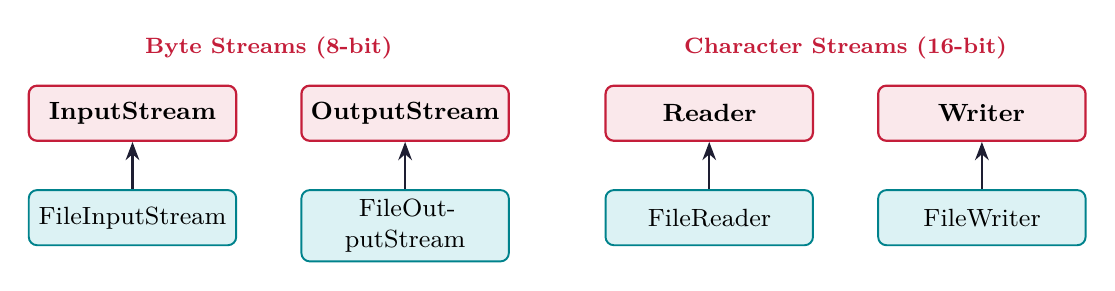
\begin{tikzpicture}[node distance=0.8cm and 1.2cm,
  base/.style={rectangle, draw=myred, fill=hdrred, text width=2.4cm,
    align=center, minimum height=0.7cm, font=\small\bfseries, rounded corners=3pt, line width=0.8pt},
  sub/.style={rectangle, draw=myteal, fill=hdrteal, text width=2.4cm,
    align=center, minimum height=0.7cm, font=\small, rounded corners=3pt, line width=0.7pt}]

  % Byte Streams
  \node[base] (is) {InputStream};
  \node[sub, below=0.6cm of is] (fis) {FileInputStream};
  \draw[arrow] (fis) -- (is);
  
  \node[base, right=0.8cm of is] (os) {OutputStream};
  \node[sub, below=0.6cm of os] (fos) {FileOutputStream};
  \draw[arrow] (fos) -- (os);

  % Character Streams
  \node[base, right=1.2cm of os] (rd) {Reader};
  \node[sub, below=0.6cm of rd] (fr) {FileReader};
  \draw[arrow] (fr) -- (rd);
  
  \node[base, right=0.8cm of rd] (wr) {Writer};
  \node[sub, below=0.6cm of wr] (fw) {FileWriter};
  \draw[arrow] (fw) -- (wr);

  % Labels
  \node[above=0.2cm of $(is.north)!0.5!(os.north)$, font=\footnotesize\bfseries, color=myred] {Byte Streams (8-bit)};
  \node[above=0.2cm of $(rd.north)!0.5!(wr.north)$, font=\footnotesize\bfseries, color=myred] {Character Streams (16-bit)};
\end{tikzpicture}
\end{tcolorbox}

% ===============================================================================
\section{Java Collections Framework}
% ===============================================================================

The Collections Framework provides a unified architecture for storing and manipulating groups of objects.

\subsection{ArrayList vs. LinkedList}

\par\noindent
{\renewcommand{\arraystretch}{1.5}%
\begin{tabularx}{\linewidth}{|B{3.2cm}|Y|Y|}
\hline
\textbf{Metric} & \textbf{\texttt{ArrayList}} & \textbf{\texttt{LinkedList}} \\
\hline
\textbf{Internal Structure} & Dynamically resizing array. & Doubly linked list. \\
\hline
\textbf{Access Time} & $O(1)$ random access (index-based). & $O(n)$ search access (sequential traverse). \\
\hline
\textbf{Insertion/Deletion} & $O(n)$ (requires element shifts). & $O(1)$ if pointer is located. \\
\hline
\textbf{Memory Overhead} & Low (only stores elements). & Higher (stores element and prev/next links). \\
\hline
\end{tabularx}}

\begin{tcolorbox}[tikzbox, title={ArrayList vs. LinkedList Memory Layout}]
\centering
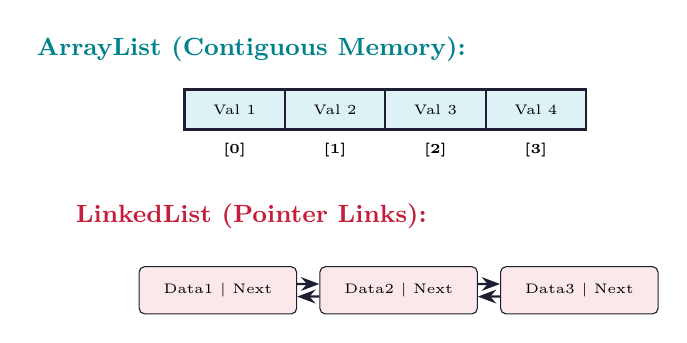
\begin{tikzpicture}[scale=0.85]
  % ArrayList
  \node[font=\small\bfseries, color=myteal] at (1,2) {ArrayList (Contiguous Memory):};
  \draw[draw=mydark, fill=hdrteal, line width=1pt] (0,0.8) rectangle (6,1.4);
  \foreach \x in {1.5, 3.0, 4.5} {
    \draw[line] (\x, 0.8) -- (\x, 1.4);
  }
  \node[font=\tiny] at (0.75, 1.1) {Val 1};
  \node[font=\tiny] at (2.25, 1.1) {Val 2};
  \node[font=\tiny] at (3.75, 1.1) {Val 3};
  \node[font=\tiny] at (5.25, 1.1) {Val 4};

  \node[font=\tiny\bfseries] at (0.75, 0.5) {[0]};
  \node[font=\tiny\bfseries] at (2.25, 0.5) {[1]};
  \node[font=\tiny\bfseries] at (3.75, 0.5) {[2]};
  \node[font=\tiny\bfseries] at (5.25, 0.5) {[3]};

  % LinkedList
  \node[font=\small\bfseries, color=myred] at (1,-0.5) {LinkedList (Pointer Links):};
  
  \node[draw=mydark, fill=hdrred, minimum width=2.0cm, minimum height=0.6cm, rounded corners=2pt] (n1) at (0.5,-1.6) {\tiny Data1 | Next};
  \node[draw=mydark, fill=hdrred, minimum width=2.0cm, minimum height=0.6cm, rounded corners=2pt] (n2) at (3.2,-1.6) {\tiny Data2 | Next};
  \node[draw=mydark, fill=hdrred, minimum width=2.0cm, minimum height=0.6cm, rounded corners=2pt] (n3) at (5.9,-1.6) {\tiny Data3 | Next};

  \draw[arrow, transform canvas={yshift=0.08cm}] (n1) -- (n2);
  \draw[arrow, transform canvas={yshift=-0.08cm}] (n2) -- (n1);
  \draw[arrow, transform canvas={yshift=0.08cm}] (n2) -- (n3);
  \draw[arrow, transform canvas={yshift=-0.08cm}] (n3) -- (n2);
\end{tikzpicture}
\tcbset{after={\color{black}}}
\end{tcolorbox}

\newpage
% ===============================================================================
\begin{center}
  {\large\bfseries\color{myred} Quick Revision --- Module 4}\\[3pt]
  {\small\color{mydark} Exception Handling, Strings, I/O Streams \& Collections $|$ OE-EC704A}
\end{center}
\noindent{\color{myred}\rule{\linewidth}{1.2pt}}
\vspace{4pt}

\begin{tcolorbox}[formulabox, title={\textbf{Exception, File I/O \& Collections Syntax}}]
{\renewcommand{\arraystretch}{1.3}%
\begin{tabularx}{\linewidth}{l Y}
\textbf{Concept} & \textbf{Syntax and Example Usage} \\
\hline
Try-Catch Block & \texttt{try \{ int a = 5/0; \} catch(ArithmeticException e) \{ ... \}} \\
Throws Declaration & \texttt{void readFile() throws IOException \{ ... \}} \\
Custom Exception & \texttt{class MyException extends Exception \{ MyException(String s)\{super(s);\} \}} \\
Buffer Reader I/O & \texttt{BufferedReader br = new BufferedReader(new InputStreamReader(System.in));} \\
\hline
\textbf{Collections \& Strings} & \textbf{Core Declarations \& Queries} \\
\hline
ArrayList Declare & \texttt{ArrayList<String> list = new ArrayList<String>();} \\
Collection Iterator & \texttt{Iterator<String> itr = list.iterator(); while(itr.hasNext()) \{ ... \}} \\
String Concat & \texttt{String s = "Biraj" + " Sarkar"; // SCP optimization} \\
StringBuffer Append & \texttt{StringBuffer sb = new StringBuffer("CGE"); sb.append("C");} \\
\end{tabularx}}
\end{tcolorbox}

\begin{tcolorbox}[defbox, title={\textbf{One-Line Definitions}}]
\begin{itemize}[leftmargin=*, itemsep=2pt]
  \item \textbf{Checked Exception:} An exception subclass checked during compilation that requires explicit handling.
  \item \textbf{Unchecked Exception:} RuntimeException subclasses resulting from logical design faults.
  \item \textbf{Immutability:} State constraint preventing modification of heap values after initial allocation.
  \item \textbf{Stream:} Abstract communication pipe that handles sequential transfer of data bytes.
  \item \textbf{Byte Stream:} Stream subclass designed to process binary data using 8-bit units.
  \item \textbf{Character Stream:} Stream subclass designed to process Unicode text data using 16-bit units.
  \item \textbf{Collections Framework:} Framework of interfaces and classes for managing structures.
  \item \textbf{Iterator:} Universal collection interface cursor that iterates elements in a forward direction.
\end{itemize}
\tcbset{after={\color{black}}}
\end{tcolorbox}

\begin{tcolorbox}[exambox, title={\textbf{Frequently Asked / Viva Questions}}]
\begin{enumerate}[leftmargin=*, label=\textbf{Q\arabic*.}, itemsep=5pt]
  \item \Q{What is the difference between \texttt{final}, \texttt{finally}, and \texttt{finalize}?}
        \texttt{final} is a modifier indicating that a class cannot be inherited, a method cannot be overridden, or a variable cannot be reassigned. \texttt{finally} is a block accompanying a try-catch block to execute clean-up operations. \texttt{finalize} is a method invoked by the Garbage Collector before reclaiming an object.
        
  \item \Q{Can we write a try block without a catch block? If so, how?}
        Yes, a try block can be followed by a \texttt{finally} block instead of a catch block. Additionally, Java 7 supports the \textbf{try-with-resources} statement, which automatically closes resources without requiring an explicit catch or finally.
        
  \item \Q{What is try-with-resources statement?}
        It is a try block declared with one or more resources (e.g., streams). The resources must implement \texttt{java.lang.AutoCloseable}. They are automatically closed when exiting the try block.
        
  \item \Q{Why are String objects immutable while StringBuffer objects are mutable?}
        Strings are cached in the String Constant Pool to save memory and ensure thread safety. StringBuffer is designed for dynamic character manipulation without creating multiple garbage references.
        
  \item \Q{What is the difference between \texttt{equals()} and \texttt{==} when comparing strings?}
        \texttt{==} compares reference equality (whether they point to the exact same object reference). The \texttt{equals()} method compares value equality (whether the character sequences are identical).
        
  \item \Q{What is the difference between byte stream classes and character stream classes?}
        Byte stream classes read and write raw 8-bit bytes (binary), whereas character stream classes read and write 16-bit Unicode characters, handling text encoding automatically.
        
  \item \Q{Why do we wrap a \texttt{FileReader} inside a \texttt{BufferedReader}?}
        Wrapping inside a \texttt{BufferedReader} reduces disk I/O requests by reading data blocks into an internal buffer. It also provides the convenient \texttt{readLine()} method.
        
  \item \Q{What is the difference between \texttt{ArrayList} and \texttt{Vector}?}
        \texttt{ArrayList} is non-synchronized, fast, and not thread-safe. \texttt{Vector} is synchronized, has thread-safe methods, and carries a significant performance overhead.
        
  \item \Q{Why does a LinkedList consume more memory than an ArrayList?}
        An ArrayList stores elements contiguously inside a backing array. A LinkedList stores elements inside node wrappers that also hold memory addresses for the previous and next nodes.
        
  \item \Q{How does the \texttt{throws} keyword differ from the \texttt{throw} keyword?}
        \texttt{throw} is used to explicitly throw a single exception instance inside a method block. \texttt{throws} is used in a method declaration to list possible checked exceptions.
\end{enumerate}
\end{tcolorbox}

\begin{tcolorbox}[tikzbox, title={Comparison: Try-Catch-Finally vs. Try-With-Resources}]
\centering
{\renewcommand{\arraystretch}{1.45}%
\begin{tabularx}{\linewidth}{|B{3.2cm}|Y|Y|}
\hline
\textbf{Metric} & \textbf{Standard Try-Catch-Finally} & \textbf{Try-With-Resources (Java 7+)} \\
\hline
\textbf{Resource Closing} & Manual (must write stream close calls in finally). & Automatic (handled by compiler behind the scenes). \\
\hline
\textbf{Boilerplate Code} & High (requires nested try-catch blocks in finally). & Minimal (declared inside try parameters). \\
\hline
\textbf{Exception Suppression} & Primary exception can be lost if close fails. & Retains primary exception; close errors suppressed. \\
\hline
\textbf{Target Classes} & Any standard classes. & Only classes implementing \texttt{AutoCloseable}. \\
\hline
\end{tabularx}}
\end{tcolorbox}

\end{document}
